\documentclass{article}
\usepackage{tikz}
\usetikzlibrary{positioning,shapes,arrows}

%%%%%%%%%Control blocks shortcuts
\tikzstyle{block} = [draw, minimum width = 2cm, minimum height = 1.2cm, fill=blue!5]
\tikzstyle{sum} = [draw, fill=blue!5, circle, node distance=1cm]
%%%%%%%%%

\begin{document}
\begin{figure}[h]\centering
    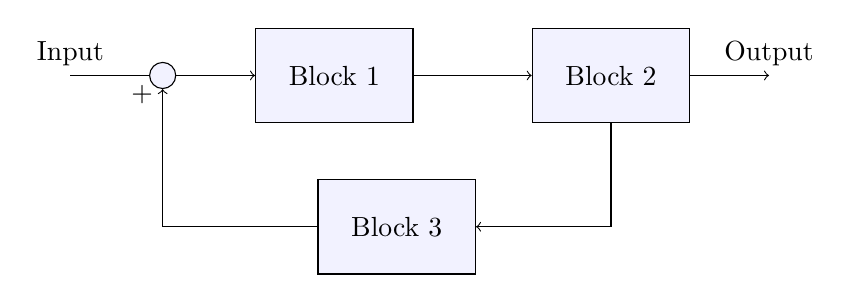
\begin{tikzpicture}
        %Blocks
        \node [block] (block1) at (0,0) {Block 1};
        \node [block, right = 1.5 cm of block1] (block2) {Block 2};
        \node [block, below left = 1 cm of block2] (block3) {Block 3} ;
        \node [sum, left = of block1] (sum1) {};
        %Arrows
        \draw[->] (block1) -- (block2);
        \draw[->] (block2.east) -- ++(1.0,0) node [right,above](){Output};
        \draw[->] (block2.south) |- (block3.east) ;
        \draw[->] (block3.west) -| (sum1) node[below left](){+};
        \draw[->] (sum1.west) ++ (-1,0) node[above](){Input}-- (sum1.west)
            (sum1.east) -- (block1.west)
        ;
    \end{tikzpicture}
    \end{figure}
\end{document}